\newpage
\subsection{Messung an Spule}\label{sec:2-2}
\subsubsection{Aufgabenstellung}

In diesem Versuchsteil soll mit Hilfe einer Maxwell-Wien-Brücke die Induktivität und der Wirkwiderstand einer vom Übungsleiter bereitgestellten RL-Schaltung bestimmt werden. Der Abgleich der Brücke erfolgt, bis am Nullindikator kein Spannungsausschlag mehr erkennbar ist, wodurch sich die unbekannten Parameter der Spule berechnen lassen.

\subsubsection{Verwendetes Material}

\begin{table}[h]
	\centering
	\caption{Verwendetes Material}
	\begin{tabularx}{\textwidth}{XXX}
		\textbf{Material} & \textbf{Verwendung} & \textbf{Anmerkungen} \\ \midrule
		                  &                     &                      \\
		                  &                     &                      \\
		                  &                     &                      \\
	\end{tabularx}
\end{table}

\subsubsection{Versuchsaufbau}

\textbf{Geräte Einstellungen}

\begin{minipage}[t]{.48\textwidth}
	Labornetzteil:
	\begin{itemize}[noitemsep]
		\item Spannung:
		\item Strom:
		\item Toleranz:
	\end{itemize}
\end{minipage}\hfill
\begin{minipage}[t]{.48\textwidth}
	Multimeter:
	\begin{itemize}[noitemsep]
		\item Einstellung: (Ohm, Volt, Ampere)
		\item Messbereich:
		\item Garantiefehlergrenzen:
	\end{itemize}
\end{minipage}

\textbf{Messschaltung}
\begin{figure}[h]
	\centering
	\begin{circuitikz}[scale=0.9, transform shape]
		\draw (0,4) to[open, v=$U_H$, o-o] (0,0)
		-- ++(3, 0) coordinate (k1)
		to[vR=$R_2$,*-] ++(0,2) coordinate (k2)
		to[R=$R_1$,-*] ++(0,2) coordinate (k3)
		-- ++(-3,0);
		\draw (k1) -- ++(3,0)
		to[vR=$R_4$] ++(0,2) coordinate (k4)
		to[vR=$R_3$] ++(0,2) -- ++(-3,0);
		\draw (k2) to[ai, v^=$U_0$, i>^=$I_0$, *-*] (k4);
		\draw (1.5,0) to[vC=$C_2$,*-] ++(0,2) coordinate (c1) -- (k2);
		\draw (c1) to[C=$C_1$,*-*] ++(0,2);
		\node[yshift=-20pt] at ($(k2)!0.5!(k4)$) {$R_0$};
	\end{circuitikz}
	\caption{Schaltung}
\end{figure}

\begin{figure}
	\begin{center}
		\includegraphics[width=0.55\textwidth]{images/Rl-Abgleich.JPG}
	\end{center}
	\caption{}\label{fig:rl-abgleich-oszi}
\end{figure}



% \begin{figure}[h]
% 	\begin{minipage}[position]{0.48\textwidth}
% 		\centering
% 		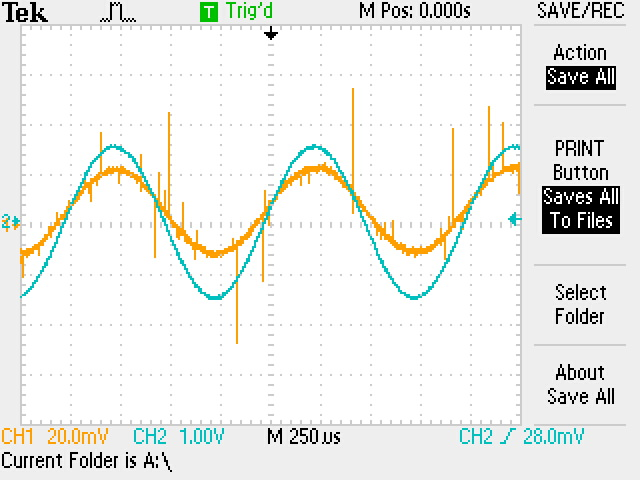
\includegraphics[height=4.5cm]{images/RC-Abgleich.JPG}
% 		\caption{Spannungsdreieck des Kondensators}
% 	\end{minipage}\hfill
% 	\begin{minipage}[position]{0.48\textwidth}
% 		\centering
% 		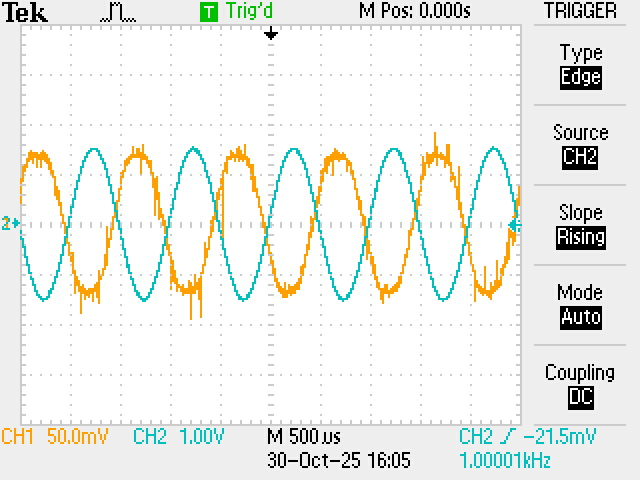
\includegraphics[height=4.5cm]{images/RL-Abgleich.JPG}
% 		\caption{Spannungsdreieck der Spule}
% 	\end{minipage}
% \end{figure}


\subsubsection{Erkenntnisse}

